\title{Homework 5 Solutions for Computer Logic and Circuit Design: PHYS306/COSC330}
\author{Dr. Jordan Hanson - Whittier College Dept. of Physics and Astronomy}
\date{\today}
\documentclass[10pt]{article}
\usepackage[a4paper, total={18cm, 27cm}]{geometry}
\usepackage{graphicx}
\usepackage{amsmath}
\begin{document}
\maketitle

\section{7-1: Latches}

\begin{enumerate}
\item Exercise 1: The active-LOW SR latch begins in the RESET state, and is SET, RESET, ...
\begin{figure}[ht]
\centering
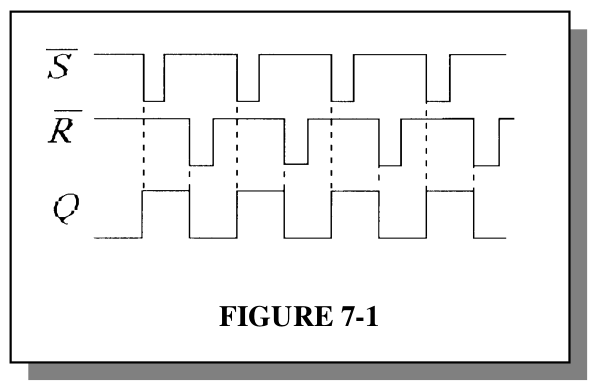
\includegraphics[width=0.35\textwidth]{exercise1_ch7.png}
\caption{\label{fig:ex1} Solution to exercise 1.}
\end{figure}
\item Exercise 2: The SR latch is now active-HIGH.  Whenever it's in the SET state and S goes high again, there is no change in the state.
\begin{figure}[ht]
\centering
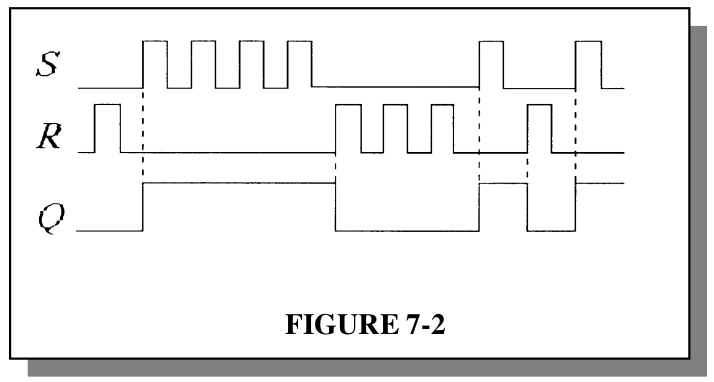
\includegraphics[width=0.35\textwidth]{exercise2_ch7.png}
\caption{\label{fig:ex2} Solution to exercise 2.}
\end{figure}
\item Exercise 4: The key here is that once the latch is SET, it stays set regardless of EN.
\begin{figure}[hb]
\centering
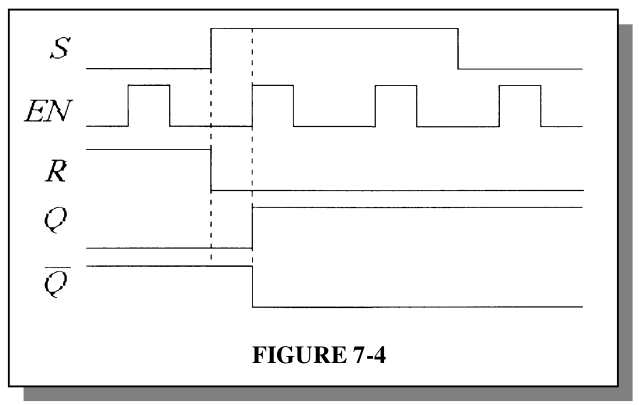
\includegraphics[width=0.35\textwidth]{exercise4_ch7.png}
\caption{\label{fig:ex4} Solution to exercise 4.}
\end{figure}
\clearpage
\item Exercise 7: For Q to be HIGH we need to enable and SET the latch.  Once it's set it stays SET until enabled and RESET.
\begin{figure}[hb]
\centering
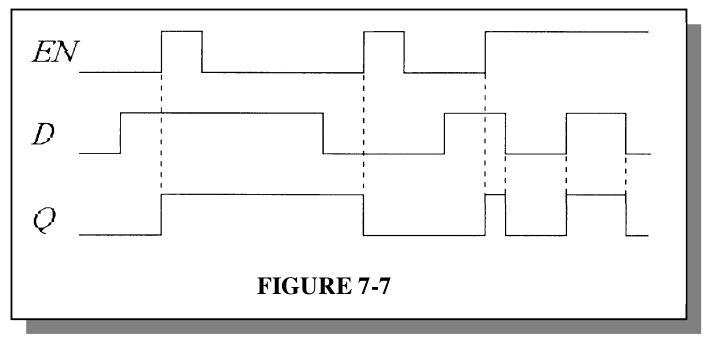
\includegraphics[width=0.4\textwidth]{exercise7_ch7.png}
\caption{\label{fig:ex7} Solution to exercise 7.}
\end{figure}
\end{enumerate}

\section{7-2: Flip-flops}

\begin{enumerate}
\item Exercise 8: The pulse-transition-detector inside each means these are synchronous devices, but (a) triggers on the negative edges and (b) triggers on positive edges of the clock.  Each device is SET, RESET, and SET again, however, these transitions line up with the negative or positive edges of CLK.
\begin{figure}[ht]
\centering
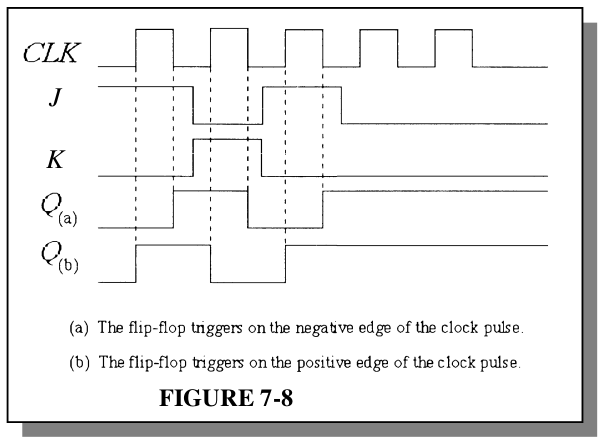
\includegraphics[width=0.35\textwidth]{exercise8_ch7.png}
\caption{\label{fig:ex8} Solution to exercise 8.}
\end{figure}
\item Exercise 12: The D flip-flop is positive edge triggered, and Q follows D only on the right posedge signals.
\begin{figure}[ht]
\centering
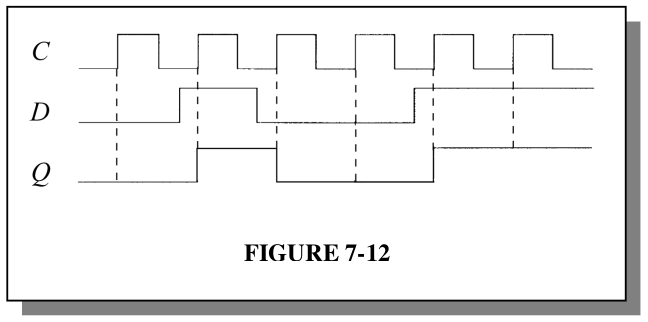
\includegraphics[width=0.35\textwidth]{exercise12_ch7.png} \hspace{0.2cm}
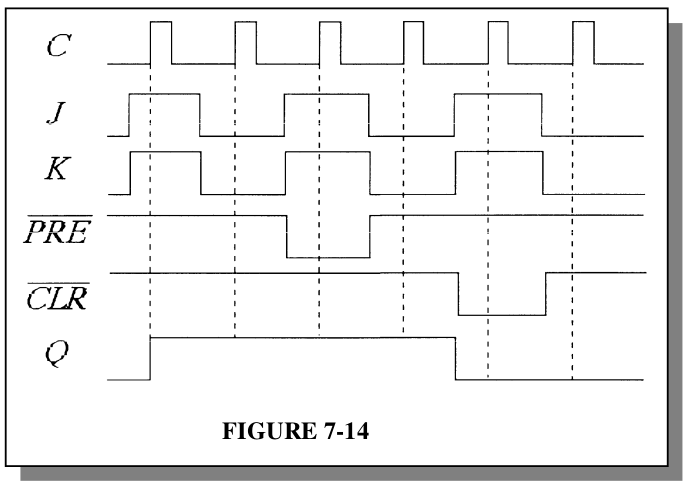
\includegraphics[width=0.35\textwidth]{exercise14_ch7.png}
\caption{\label{fig:ex12} (Left) Solution to exercise 12. (Right) Solution to exercise 14.}
\end{figure}
\item Exercise 14: The J and K inputs act together, alternatively toggling and indicating no-change.  However, when the preset signal is active-LOW, the JK flip-flop is SET, and when the clear signal is active-LOW, the unit is RESET.
\end{enumerate}

\section{7-3: Flip-flop operating characteristics}

\begin{enumerate}
\item Adding the two numbers gives the minimum period of 67 ns.  Inverting the number gives the frequency: $1/(67)$ ns$^{-1} = 0.0149$ GHz$ = 14.9$ MHz.
\end{enumerate}

\section{7-4: Flip-flop Applications}

\begin{enumerate}
\item Exercise 25: Because the flip-flop has to wait until the next posedge to go HIGH after the $\bar{Q}$ output RESETs it, the $Q$ output remains high for a clock cycle and low for a subsequent clock cycle.  Thus, this is a frequency divider (by 2).
\begin{figure}[ht]
\centering
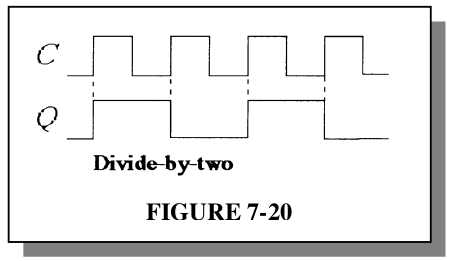
\includegraphics[width=0.35\textwidth]{exercise25_ch7.png}
\caption{\label{fig:ex25} The solution to exercise 25.}
\end{figure}
\end{enumerate}
\end{document}
